\documentclass[final]{article}

% Use the official APS360 style when it is available in the course template.
% The fallback only makes this draft compile locally.
\IfFileExists{APS360.sty}{\usepackage{APS360}}{
  \usepackage[margin=0.68in]{geometry}
  \usepackage{times}
}
\usepackage[utf8]{inputenc}
\usepackage[T1]{fontenc}
\usepackage{hyperref}
\usepackage{url}
\usepackage{booktabs}
\usepackage{amsmath}
\usepackage{microtype}
\usepackage{xcolor}
\usepackage{graphicx}
\usepackage{tikz}
\usetikzlibrary{arrows.meta,positioning,fit}
\usepackage[numbers,sort&compress]{natbib}

\definecolor{deepblue}{HTML}{244B78}
\definecolor{lightblue}{HTML}{E9F2FA}
\definecolor{lightgreen}{HTML}{E9F6EE}
\definecolor{lightorange}{HTML}{FFF1DF}
\definecolor{lightpurple}{HTML}{F0EAF8}
\hypersetup{colorlinks=true,linkcolor=deepblue,citecolor=deepblue,urlcolor=deepblue}

\title{\vspace{-0.35in}\textbf{Can a 100M-Parameter Transformer Learn\\
Simple Python Programming Tasks?}}

\author{
  George Yuan\\
  1012152224, \href{mailto:zhijie.yuan@mail.utoronto.ca}{zhijie.yuan@mail.utoronto.ca}\\
  GitHub: \url{https://github.com/ShiinaMahiruOvO/aps360-small-code-lm}
}
\date{}

\begin{document}
\maketitle
\vspace{-0.38in}

\section*{Introduction}
Large code models can solve complex programming problems, but their scale makes it difficult to determine how much ability can be learned with a course-project compute budget. This project asks whether a decoder-only Transformer with approximately 100 million parameters, pretrained from scratch on Python code, can generate correct solutions to beginner-level programming tasks. These tasks include basic string and collection manipulation, linear scans and simple algorithms, and introductory data-structure operations such as binary search tree queries.

Our main architectural improvement is a \emph{looped Transformer} that applies a shared group of layers more than once. This increases effective computational depth without proportionally increasing the number of parameters. We compare it with a standard Transformer trained on the same data and evaluate both models by running generated programs against hidden unit tests. Deep learning is appropriate because natural-language specifications and programs are variable-length sequences with many valid implementations, making fixed rules or templates too brittle. Our main question is whether iterative computation improves functional correctness, especially when a task combines several individually simple requirements.

This is an individual project. I will implement and document the data pipeline, model architecture, training procedures, execution-based evaluation, and final analysis. Configuration files, fixed random seeds, and version-controlled scripts will be used to keep the experiments reproducible.

\section*{Illustration}
\vspace{-0.08in}
\begin{figure}[h]
\centering
\resizebox{0.98\linewidth}{!}{
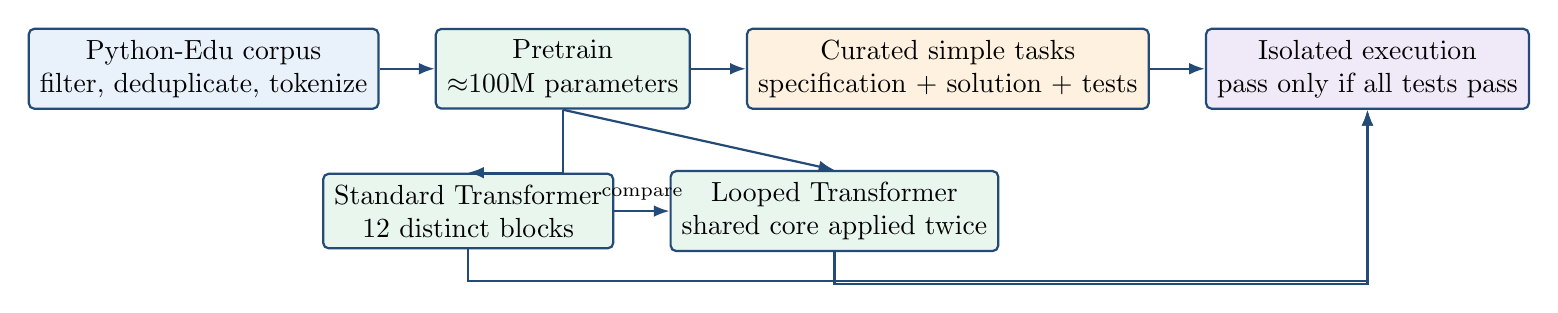
\begin{tikzpicture}[
  node distance=5mm and 7mm,
  box/.style={draw=deepblue, rounded corners=2pt, thick, align=center,
              minimum height=8mm, inner sep=4pt},
  data/.style={box, fill=lightblue},
  model/.style={box, fill=lightgreen},
  train/.style={box, fill=lightorange},
  eval/.style={box, fill=lightpurple},
  arr/.style={-{Latex[length=2mm]}, thick, draw=deepblue}
]
\node[data] (py) {Python-Edu corpus\\filter, deduplicate, tokenize};
\node[model, right=of py] (pre) {Pretrain\\$\approx$100M parameters};
\node[train, right=of pre] (bst) {Curated simple tasks\\specification + solution + tests};
\node[eval, right=of bst] (test) {Isolated execution\\pass only if all tests pass};

\draw[arr] (py) -- (pre);
\draw[arr] (pre) -- (bst);
\draw[arr] (bst) -- (test);

\node[model, below=8mm of pre, xshift=-12mm] (base) {Standard Transformer\\12 distinct blocks};
\node[model, right=of base] (loop) {Looped Transformer\\shared core applied twice};

\draw[arr] (pre.south) |- (base.north);
\draw[arr] (pre.south) -- (loop.north);
\draw[arr] (base.east) -- node[above, font=\scriptsize]{compare} (loop.west);
\draw[arr] (base.south) |- ++(0,-4mm) -| (test.south);
\draw[arr] (loop.south) |- ++(0,-4mm) -| (test.south);
\end{tikzpicture}}
\vspace{-0.08in}
\caption{Project pipeline. The standard and looped Transformers use the same tokenizer, training data, fine-tuning tasks, and execution-based evaluation.}
\label{fig:pipeline}
\vspace{-0.12in}
\end{figure}

\section*{Background \& Related Work}
The Transformer established attention-only sequence modelling and forms the basis of our decoder \citep{vaswani2017attention}; RoPE supplies position information to its attention layers \citep{su2021roformer}. Codex and HumanEval demonstrated the importance of evaluating generated code through execution rather than textual similarity \citep{chen2021evaluating}. MBPP provides short Python problems close to our intended difficulty \citep{austin2021program}, while SmolLM-Corpus provides the educational Python source used for pretraining \citep{benallal2024smollm}. Most closely related to our architectural experiment, Universal Transformers repeatedly apply shared layers and report benefits on algorithmic tasks \citep{dehghani2019universal}. We apply this general idea to small-scale code generation and compare it directly with a conventional Transformer.

\section*{Data Processing}
For pretraining, we use the Python-Edu subset of SmolLM-Corpus \citep{benallal2024smollm}. It contains Python files selected for educational quality. Our pipeline removes malformed, generated, extremely short, and duplicate files; checks that retained samples parse as Python; and separates repositories between training and validation to reduce leakage. We train an 8,192-token byte-pair tokenizer on the cleaned text and convert the corpus into memory-mapped token shards. The processed corpus contains approximately 498 million training tokens and 55 million validation tokens.

For supervised fine-tuning, we combine easy problems filtered from KodCode-Light-RL-10K \citep{kodcode2025light} with tasks generated by us. The task groups cover basic strings and collections, simple counting/searching/sorting algorithms, and introductory data structures. Our generated BST subset provides a controlled structured case study with prompts, reference solutions, and unit tests. We remove incomplete problems, invalid reference code, answer leakage, and duplicate statements or solutions. Training, validation, and evaluation sets are separated before prompt variants are produced. Evaluation uses a reviewed easy subset of MBPP and held-out generated tasks, with overlap removed from the fine-tuning data. Reference solutions must pass their tests before inclusion, and generated programs are executed in an isolated environment with time and resource limits.

\section*{Architecture}
The baseline is a decoder-only Transformer with an 8,192-token vocabulary, context length 1,024, hidden width 768, 12 layers, 12 attention heads, RMSNorm, RoPE, and SwiGLU, totalling approximately 97.5M parameters. It is pretrained with next-token prediction and then supervised on instruction--solution pairs.

The looped model keeps two input blocks and two output blocks, while its eight middle blocks form a shared core that is executed twice. It therefore retains approximately the same number of distinct parameters as the baseline but has an effective depth of 20 layers. This provides a controlled test of whether a small model benefits more from iterative computation than from using each parameter only once. If time permits, we will test lightweight iteration-specific adapters and execution-based reinforcement learning as secondary extensions.

\section*{Baseline Model}
The standard 12-layer Transformer is the primary baseline. It uses the same tokenizer, pretraining corpus, fine-tuning data, optimizer, and decoding settings as the looped model, making the architecture the main experimental variable. Functional correctness is measured with pass@1: a task passes only when the generated program satisfies every hidden test. We will report overall results, results by task group, parameter count, and training and inference cost. A small public code model may also be included as an external reference, but the parameter-matched standard Transformer remains the main comparison.

\section*{Ethical Considerations}
Public code can contain licensing, attribution, privacy, and memorization risks, so we document dataset provenance and remove duplicates where possible. Generated programs may be incorrect or insecure; this model is an educational prototype, not a deployment-ready programming assistant. Untrusted completions are executed only in an isolated environment without network access. We will report failures and possible benchmark contamination and avoid claims beyond the beginner-level tasks studied here.

\newpage
\bibliographystyle{plainnat}
\bibliography{references}

\end{document}
